\documentclass[tikz,border=10pt]{standalone}
\usepackage{tikz}
\usetikzlibrary{arrows.meta,positioning}
\usepackage{xcolor}
\renewcommand{\familydefault}{\sfdefault}
\pagecolor{gray!8}

\begin{document}
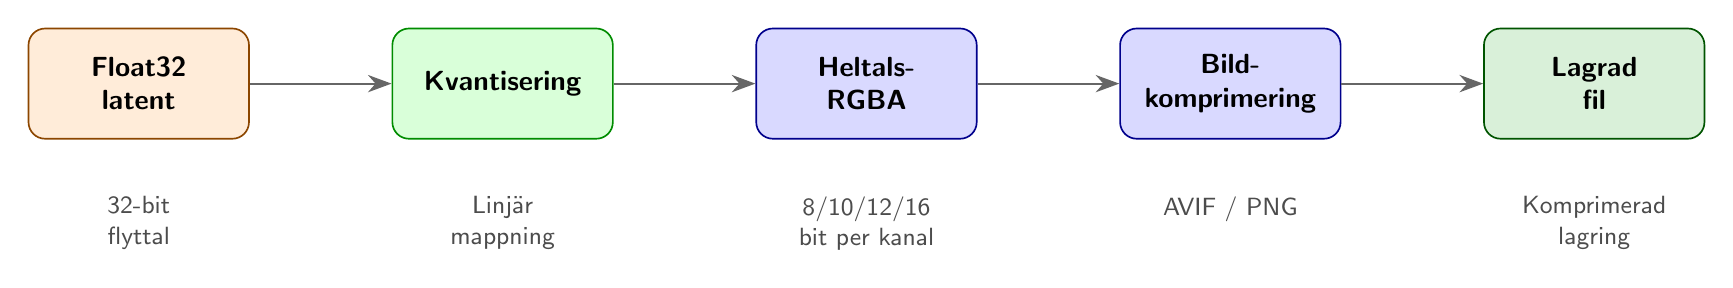
\begin{tikzpicture}[
  >=Stealth,
  box/.style={
    rounded corners=6pt,
    minimum width=28mm,
    minimum height=14mm,
    draw=#1!55!black,
    line width=0.6pt,
    fill=#1!15!white,
    font=\sffamily\bfseries\normalsize,
    align=center,
    inner sep=4pt,
  },
  arr/.style={
    -{Stealth[length=3mm,width=2.2mm]},
    line width=0.8pt,
    black!60,
  },
  note/.style={
    font=\sffamily\small,
    text=black!70,
    align=center,
  },
]

% Nodes
\node[box=orange] (latent) {Float32\\latent};

\node[box=green, right=18mm of latent] (quant) {Kvantisering};

\node[box=blue, right=18mm of quant] (rgba) {Heltals-\\RGBA};

\node[box=blue, right=18mm of rgba] (compress) {Bild-\\komprimering};

\node[box=green!60!black, right=18mm of compress] (file) {Lagrad\\fil};

% Arrows
\draw[arr] (latent)   -- (quant);
\draw[arr] (quant)    -- (rgba);
\draw[arr] (rgba)     -- (compress);
\draw[arr] (compress) -- (file);

% Annotations below
\node[note, below=6mm of latent]   {32-bit\\flyttal};
\node[note, below=6mm of quant]    {Linjär\\mappning};
\node[note, below=6mm of rgba]     {8/10/12/16\\bit per kanal};
\node[note, below=6mm of compress] {AVIF / PNG};
\node[note, below=6mm of file]     {Komprimerad\\lagring};

\end{tikzpicture}
\end{document}
